
% The \phantomsection command is needed to create a link to a place in the document that is not a
% figure, equation, table, section, subsection, chapter, etc.
% https://tex.stackexchange.com/questions/44088/when-do-i-need-to-invoke-phantomsection
\phantomsection

% Multiple-language document - babel - selectlanguage vs begin/end{otherlanguage}
% https://tex.stackexchange.com/questions/36526/multiple-language-document-babel-selectlanguage-vs-begin-endotherlanguage
\begin{otherlanguage*}{english}

% The \phantomsection command is needed to create a link to a place in the document that is not a
% figure, equation, table, section, subsection, chapter, etc.
% https://tex.stackexchange.com/questions/44088/when-do-i-need-to-invoke-phantomsection
\phantomsection

% Multiple-language document - babel - selectlanguage vs begin/end{otherlanguage}
% https://tex.stackexchange.com/questions/36526/multiple-language-document-babel-selectlanguage-vs-begin-endotherlanguage
\begin{otherlanguage*}{brazil}

\chapter{\lang{Experimental Analysis}{Análise Experimental}} \label{cap:analise:experimental}

Este capítulo apresenta a análise experimental sobre o Serviço criado. Para que seja possível
validar o Serviço uma aplicação de testes foi criada em Go, que é um acrescentador de valores
em memória. Sempre que uma requisição chega a ele, este incrementa um no seu valor em memória.
Esta é uma aplicação \textit{Stateful} e, portanto, é passível de ser utilizada no nosso Serviço.
Este capítulo pretende responder a algumas perguntas a partir da análise dos experimentos:

\begin{itemize}
	\item Existe impacto ao se utilizar o Interceptador para interceptar requisições à
	aplicação alvo? Este impacto deve ser considerado ao se utilizar o Serviço nas
	aplicações.
	\item Qual o impacto de tempo para a aplicação ser restaurada com a implementação do
	\textit{Checkpoint/Restore} com técnicas de \textit{Event Sourcing}?
	\item Qual o impacto geral na vazão e latência da aplicação quando ela está sendo
	interceptada pelo Interceptador? Qual a vazão e latência da aplicação quando ela
	está sendo executada \textit{standalone}? Há um impacto pela adição do Interceptador?
	\item Qual a latência da aplicação durante a recuperação da aplicação pelas técnicas de
	\textit{Event Sourcing}?
\end{itemize}

Para responder estas perguntas fizemos primeiro uma instrumentação no Serviço para que
pudessemos coletar pontos importante para análise, como, por exemplo, momentos em que a
aplicação alterou o estado do Interceptador, momento da introdução da falha do Interceptador,
momento da detecção pelo Administrador de Estado e tempo até a aplicação retornar ao estado
de Pronto. A análise de teste de carga para determinar a vazão e latência das requisições com
diferentes cargas no sistema. A partir disto pretendemos responder as perguntas para esta
análise. É importante destacar, que como a aplicação executa no mesmo nó, não há perdas
significativas de latência para comunicação entre serviços.

Para realizar o teste de carga, utilizamos a aplicação bombardier \cite{bombardier}, que
permite realizar um número arbitrário de requisições concorrentes, definindo a quantidade
de requisições e o tamanho da concorrência, que nos permite testar a aplicação sob uma
carga mais real. Para coleta de outras métricas utilizamos horário de início e fim de cada
uma das modificações. O Serviço e a aplicação executam na mesma máquina o horário é
igual para todos e não é necessário sincronização de relógios entre máquinas.

\section{Análise da inteterferência do Interceptador na aplicação}

Para fins de entender o quanto o Interceptador interfere no serviço que ele monitora,
instrumentamos a aplicação e utilizamos um teste de carga para verificar a performance
em três casos, da aplicação \textit{standalone}, isto é, sem a interferência do Interceptador,
da aplicação com o Interceptador utilizando memória para armazenamento das requisições e 
da aplicação com o Interceptador utilizando um banco de dados SQL para armazenamento das
requisições. Realizamos os mesmos testes de carga utilizando o bombardier para realizar
requisições com N clientes paralelamente durante dez segundos. A partir da finalização
das requisições obtivemos o valor de latência para o p95 da distribuição das requisições 
 pudemos construir um gŕafico de vazão por latência para os três casos, que é mostrado na Figura
\ref{fig:analysis-interceptor-standalone}.

O gŕafico da Figura \ref{fig:analysis-interceptor-standalone} nos provê informações que já
esperávamos, mas serão confirmadas por ele. Na aplicação \textit{standalone}, linha em vermelho,
podemos ver que demora muito para a aplicação atingir seu máximo de sobrecarga, somente entre
seis mil e dez mil clientes acabamos tendo uma performance que só piora a partir do aumento
da utilização do serviço. Inicialmente o serviço tem uma latência muito pequena, por exemplo,
com cinquenta clientes, temos apenas 5.11ms de latência.

A partir do momento que introduzimos o Interceptador temos uma piora, tanto da latência inicial,
quanto uma piora na questão da máxima vazão da aplicação. No caso da aplicação utilizando uma
implementação de armazenamento em memória, linha verde na Figura \ref{fig:analysis-interceptor-standalone},
temos que o máximo de carga do serviço se dá entre dois mil a dois mil e setecentos clientes
simultâneos. Há uma piora direta logo nos primeiros cinquenta clientes, onde a latência
p95 tem seu valor 38.55ms. Isto mostra que o impacto do nosso Interceptador e pelas
operações que ele faz, como, por exemplo, processamento da requisição obtendo apenas as
partes necessárias para o armazenamento, acréscimo da versão de ordem da requisição,
envio da requisição para a aplicação e posterior retorno da resposta para o cliente, geram
uma sobrecarga que influencia na performance do sistema como um todo. É importante notar que
a implementação em memória que utilizamos não tem possibilidade de realizar o \textit{Checkpoint},
já que não há memória infinita e não poderíamos armazenar todas as requisições em memória
que seriam necessárias para a reprojeção. Uma possibilidade de melhoria dessa abordagem,
que não foi feita, seria armazenar parte em memória e parte em um armazenamento fixo, como
um banco de dados ou em um arquivo.

Já na implementação do Interceptador com armazenamento em um banco de dados SQL, linha azul
na Figura \ref{fig:analysis-interceptor-standalone}, temos a pior performance de todas. Isto
se deve principalmente por dois fatores, da sobrecarga do sistema que realizamos os experimentos,
já que este estava executando o Kubernetes, um banco de dados, nosso Serviço e a aplicação
em uma máquina de 2vCPU e 4GB de memória, e também pela latência na inserção das entradas
de requisições no banco de dados. Como podemos ver na Figura \ref{fig:analysis-interceptor-standalone},
a capacidade máxima do sistema é atingida muito rapidamente, entre trezentos e quinhentos
clientes simultâneos. A aplicação também apresenta a pior performance em latência já no
começo dos experimentos com cinquenta clientes simultâneos, com uma latência de 151.94ms,
quase 400\% a mais que na implementação com o Interceptador com armazenamento em memória e
quase 3000\% a mais que na aplicação \textit{standalone}. Para utilizar essa solução em
um ambiente de produção seria necessário deixar a aplicação mais performática, através da
possibilidade de utilização de bancos mais rápidos, como de chave/valor ou de documentos.

\begin{figure}[h]
\centering
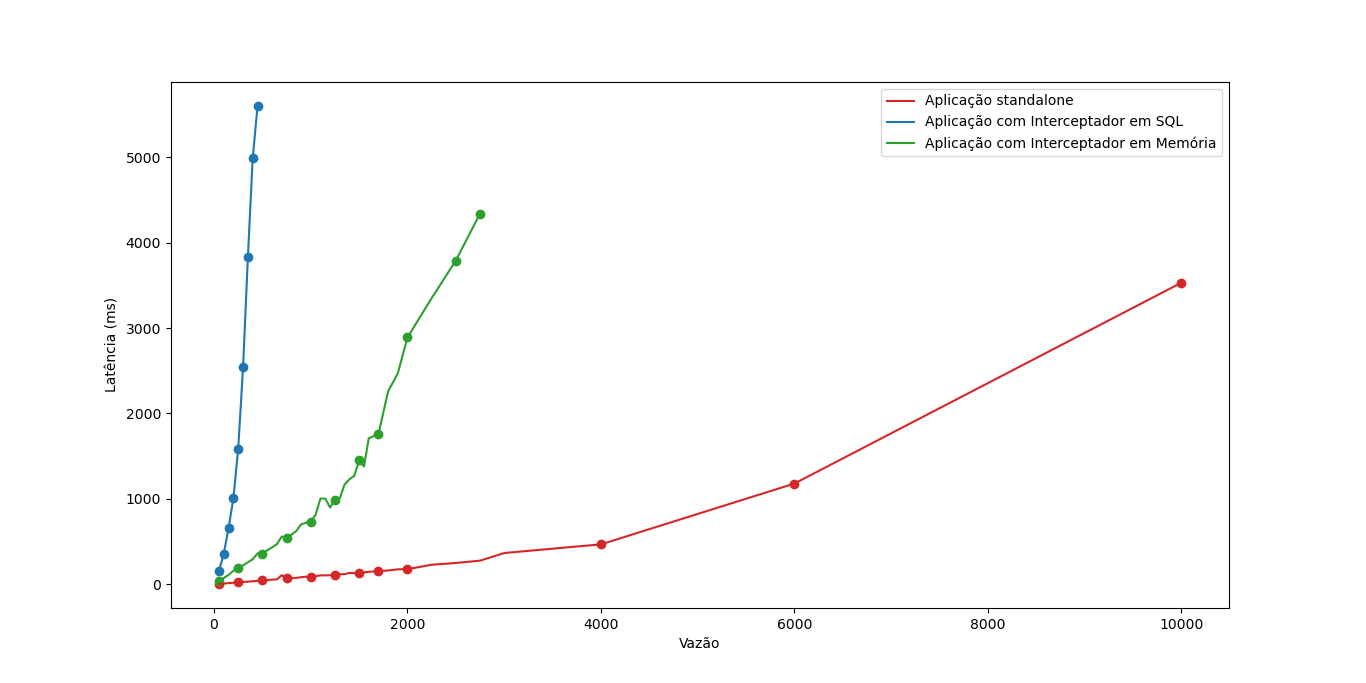
\includegraphics[scale=0.46]{images/vazaoxlatencia.png}
\caption{Gráfico de sobreposição de vazão X latência da aplicação alvo de forma \textit{standalone}, da aplicação alvo com o Interceptador com armazenamento em memória e da aplicação alvo com o Interceptador com armazenamento em banco de dados SQL.}
\label{fig:analysis-interceptor-standalone}
\end{figure}

Para nível de comparação no impacto do banco de dados na aplicação, instrumentamos o
código do Interceptador para capturar métricas sobre a latência em escrever a requisição
no banco de dados. Nas requisições com trezentos clientes simultâneos que obtemos uma
latência p95 de 1590ms, tivemos uma latência p95 para inserção da requisição no banco
de 1117ms, um impacto de cerca de 70.25\% na latência da aplicação. Uma estratégia seria combinar
a estratégia de implementação do armazenamento em memória com o armazenamento em banco de
dados SQL. Teríamos uma lista com tamanho fixo de dados, que armazenaria as requisições em
memória, onde a partir do momento em que ela excedesse sem máximo, iriamos escrever os dados no
banco de dados uma única vez, e continuariamos sobreescrevendo a lista. Com isto,
iríamos diminuir a latência de escrita, já que seria feita menos vezes e aumentar a
eficiência pelo armazenamento em memória.

\section{Análise do período de tempo de Checkpoint do Interceptador}

Nesta Seção, pretendemos discutir e analisar qual o tempo gasto pelo \textit{Checkpoint} do
Interceptador na implementação com CRIU. Na implementação com técnicas de
\textit{Event Sourcing} não temos uma alteração, por exemplo, da latência das requisições ao
se fazer um \textit{Checkpoint}, pois este ocorre passivamente. Já na implementação com CRIU
a aplicação deve ser pausada por um momento para salvamento do seu estado e isto gera uma
piora na qualidade de serviço para o usuário de maneira momentânea. Para simular este estado,
iniciamos realizando um teste de carga na aplicação para criar um estado, a partir daí, iniciamos
ao mesmo tempo um \textit{Checkpoint} a partir do Interceptador e um outro teste de carga, que deve
durar mais tempo que o \textit{Checkpoint}.

Coletamos dados para a latência das requisições que atingem o Interceptador em um período de
tempo que inclui antes de uma falha na aplicação alvo, durante a recuperação da aplicação
alvo e posteriormente da recuperação no mesmo teste. Estes testes nos proveram uma latência
p95 de 7.3s para as requisições do período de tempo, onde já existiam mil requisições
acumuladas para que ocorresse a reprojeção durante a recuperação e os tínhamos cem clientes
realizando mil requisições simultâneas para a aplicação durante o período de tempo.

Novamente, tivemos uma piora de latência do serviço, que se deve principalmente pelo fator
da nossa aplicação ter que realizar todas as requisições já feitas para a aplicação atingir
o estado antes da falha na recuperação. Na proposta de \cite{muller2022architecture} a
arquitetura realiza a poda das requisições, onde, menos requisições teriam que ser refeitas
a partir de uma falha para a recuperação através da criação de imagens de \textit{Checkpoint}
utilizando o CRIU.

\section{Análise da recuperação com técnicas de Event Sourcing}

Nesta Seção queremos investigar o impacto das técnicas de \textit{Event Sourcing} na
recuperação do estado de uma aplicação que falhou. Para isso, primeiro utilizamos nosso teste
de carga para levar a aplicação até um estado, com mil requisições(caso A), dez mil
requisições(caso B) e vinte mil requisições(caso C), com mais requisições acumuladas o serviço
degrada a ponto de não possibilitar testes com as configurações de \textit{cluster} que utilizamos.
Depois repetimos o mesmo teste com cada uma delas, ao alcançar o estado a aplicação terá uma falha
ocasionada pela interrupção da execução do container pela ferramenta crictl. Após a falha,
a recuperação deve ocorrer, neste momento, passamos a realizar um teste de carga igual para
todos os casos, cem requisições serão feitas de maneira concorrente entre dez clientes.

\begin{table}[htb]
\caption[Latência durante recuperação de requisições acumuladas.]{Latência durante recuperação de requisições acumuladas.}
\label{tab:event-sourcing-latency}
\centering
\begin{tabular}{|c|c|}
\hline
\textbf{\begin{tabular}[c]{@{}c@{}}Ńúmero de requisições\\ acumuladas\end{tabular}} & \textbf{Latência} \\ \hline
1000(A)                                                                            & 74.69ms             \\ \hline
10000(B)                                                                            & 122.76ms            \\ \hline
20000(C)                                                                               & 10010ms             \\ \hline
\end{tabular}
\end{table}

Os resultados do teste estão na Tabela \ref{tab:event-sourcing-latency}. Verificamos, que,
temos uma degradação relevante entre dez mil requisições acumuladas e vinte mil requisições
acumuladas, indo de 122.76ms de latência para 10010ms de latência para as requisições.
Novamente, quanto mais requisições acumuladas o Interceptador possui, mais demorada se torna
uma recuperação ao realizar todas as requisições novamente para a aplicação alvo. Esta análise
mostra uma premissa que já tínhamos, de que existe um limite para utilização das técnicas
de \textit{Event Sourcing} sobre o \textit{Checkpoint/Restore}, já que, conforme mais tempo
a aplicação vive, mais se torna necessário utilizar outras técnicas para ser possível reduzir
a replicação das requisições na recuperação, em \cite{muller2022architecture} a diminuição da
pilha foi feita através da implementação da recuperação com CRIU.

Agora, pretendemos também investigar o tempo que levamos entre a detecção, a recuperação e
atingir o estado de pronto em cada caso, como em \cite{vayghan2021kubernetes}, adicionamos
métricas ao controlador de Pods, para definir a detecção, e no nosso script identificamos o
início da falha, a recuperação é definida nos momentos em que se altera o estado do Interceptador
e o estado de Pronto também é instrumentado pelo controlador de Pods. Na Tabela
\ref{tab:latency-restoring} temos os valores para o início da recuperação após uma falha e o tempo
até a aplicação estar disponível novamente após a recuperação. No caso C temos um tempo muito
superior aos casos A e B, isto se deve por vários fatores, desde a configuração do nosso
\textit{cluster} que não permite escalabilidade e também da necessidade de se obter todas as
requisições de um banco de dados para replicação das requisições. A Tabela \ref{tab:latency-restoring}
demonstra que a implementação com técnicas de \textit{Event Sourcing} degrada conforme temos mais
requisições acumuladas no Interceptador para realizar a recuperação.

\begin{table}[htb]
\caption[Tempos de detecção de faha e de recuperação final de um contêiner alvo.]{Tempos de identificação de recuperação e de recuperação final de um contêiner alvo.}
\label{tab:latency-restoring}
\centering
\begin{tabular}{|c|c|c|}
\hline
\textbf{\begin{tabular}[c]{@{}c@{}}Ńúmero de requisições\\ acumuladas\end{tabular}} & \textbf{\begin{tabular}[c]{@{}c@{}}Tempo de detecção \\ (segundos) \end{tabular}} &
\textbf{\begin{tabular}[c]{@{}c@{}}Tempo de Recuperação \\ (segundos) \end{tabular}} \\ \hline
1000(A) &  0.991011s & 0.990702s \\ \hline
10000(B) & 0.998153s & 0.975395s     \\ \hline
20000(C) & 1.013021s & 856.67s \\ \hline
\end{tabular}
\end{table}

Na tabela \ref{tab:latency-restoring} percebemos que nosso limite da restauração quanto ao
número de requisições armazenadas está entre dez mil requisições e vinte mil requisições.
O aumento de cerca de 1s no tempo de restauração para cerca de 14min mostra uma perda de
performance muito grande. Seria essencial integrar outros \textit{Checkpoints} durante a
interceptação das requisições com o método de técnicas de \textit{Event Sourcing} para que
fosse possível diminuir o tempo de latência na recuperação a partir da dimunição da
quantidade de requisições armazenadas antes do último \textit{Checkpoint}.

\end{otherlanguage*}
